%This chapter focuses on the small things your plots swim in. If a line graph is a fish, the water is the 

\section{Axis Aspect and Limits}\label{sec:aspectLim}
The most basic plot is the empty plot. 

\pyfile{empty.py}

\begin{center}
    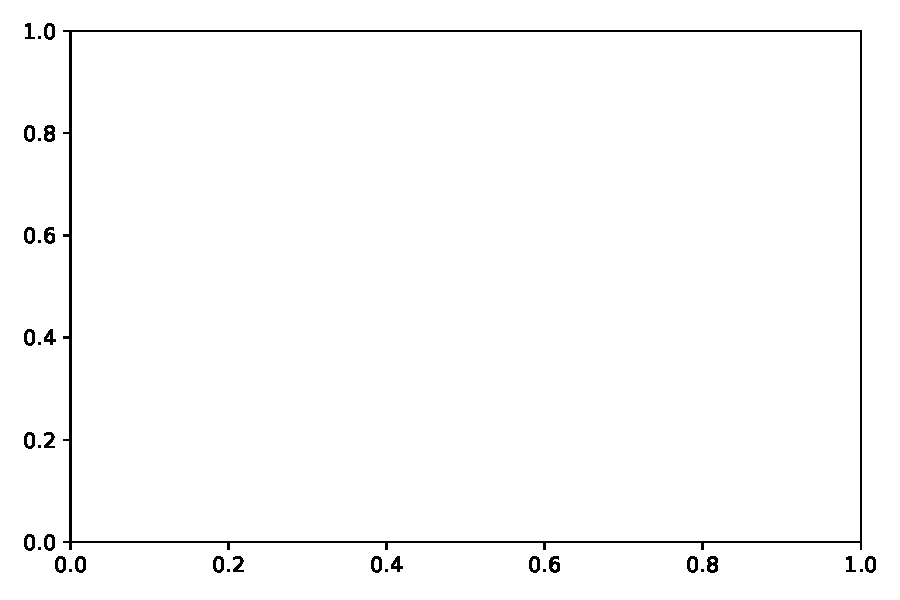
\includegraphics[width = .6\textwidth]{figures/proseplots/empty.pdf}
\end{center}


You'll notice this defaults to plotting the square region between data points (0,0) and (1,1). However, the plot is not square by default. That is to say the \emph{aspect} is not one, where the aspect is the ratio of height to width. This can be changed with the axes method \code{set_aspect()}. For equal scaling, use \code{ax.set_aspect('equal')} or \code{ax.set_aspect(1)}.

\pyfile{empty-square.py}

\begin{center}
    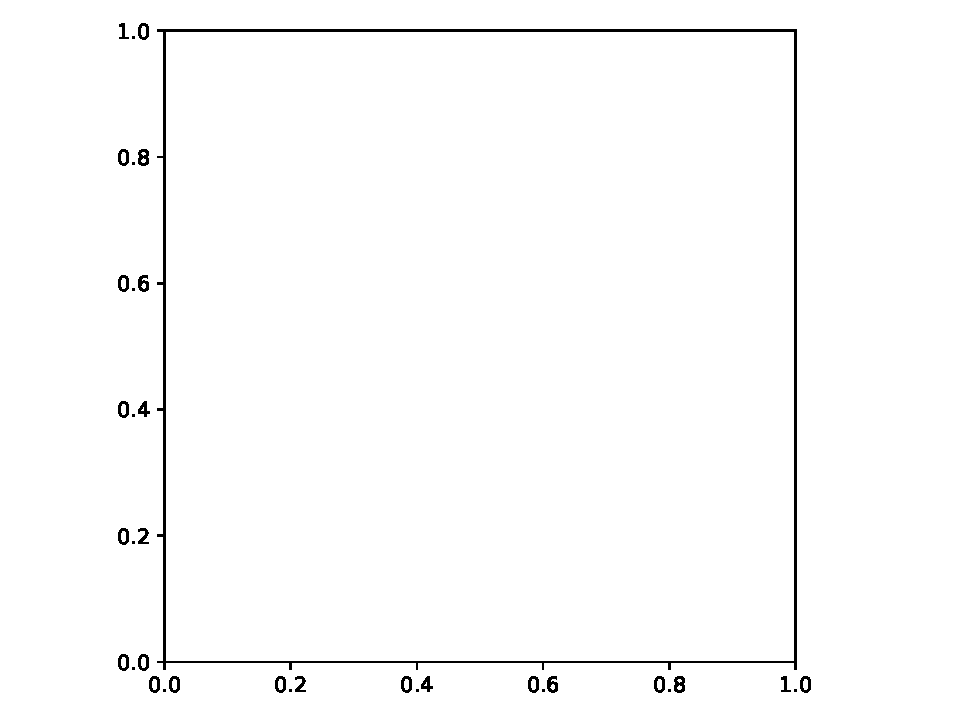
\includegraphics[width = .6\textwidth]{figures/proseplots/empty-square.pdf}
\end{center}

As we already covered in Chapter \ref{chapter:oop}, the $x$ and $y$ limits can be adjusted with axes methods \code{set_xlim()} and \code{set_ylim()}, taking a sequence for the minimum and maximum values. If you don't explicitly set the limits, matplotlib will set the limits automatically based on the data. You can retrieve those limits with the getter methods, \code{get_xlim()} and \code{get_ylim()}. 
The program below makes use of both methods. We plot a few lines, and after each plot call, matplotlib is quietly updating the axes limits. Using the \code{fill_between()} method, which creates a color fill in the defined region, the expanding limits are shown. The colors are chosen automatically by matplotlib because I haven't explicitly specified a color value. 

%I also use the \code{zorder} parameter, which specifies the ordering of the plotted objects. By default, text is plotted over lines and lines are plotted over other objects like the fill created by \code{fill_between()} (which belongs to a more general category called \emph{patches}). Within each of these three categories, objects created later in the program are plotted over previously created objects. \code{zorder} can be used to create a different ordering. Objects with a greater \code{zorder} value are ordered further to the front. Below, \code{zorder} is used to reverse the default order---the later fills are further to the back. 
% https://matplotlib.org/stable/api/_as_gen/matplotlib.axes.Axes.fill_between.html

\pyfile{expanding-lims.py}

\begin{center}
    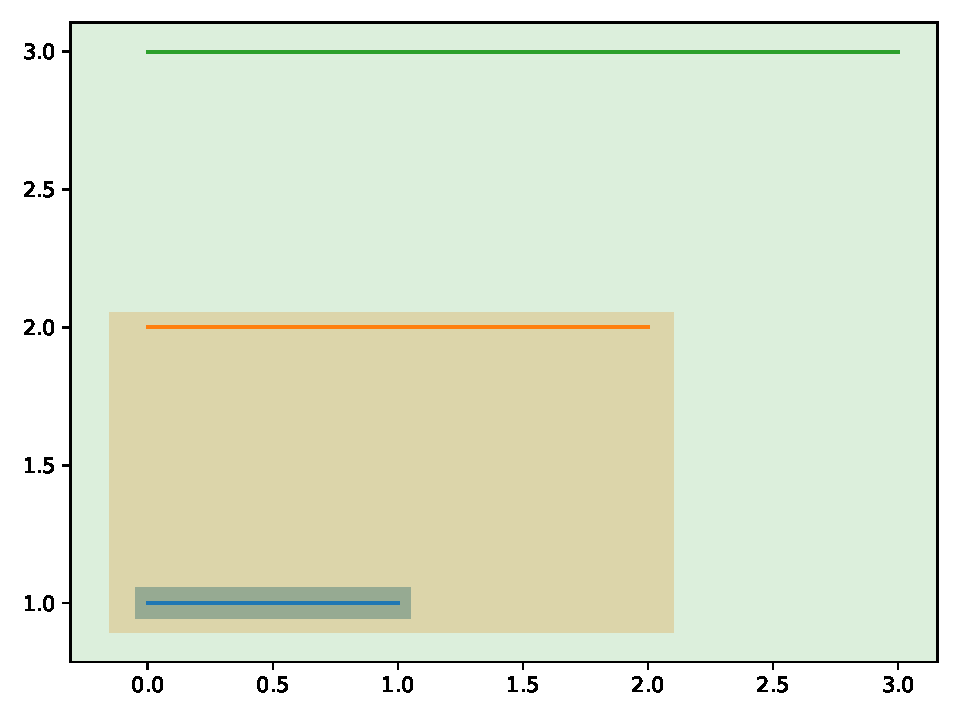
\includegraphics[width = .6\textwidth]{figures/proseplots/expanding-lims.pdf}
\end{center}

If your axes limits are too restrictive, plot elements will be cut off. If you want your plot element to break past the end of the axes, spilling into the outer figure space, you can change this by setting \code{clip_on = False} in the appropriate method. Below, we create two circles with \code{ax.plot()} and set restrictive $x$-axis limits. The first circle, in blue, would extend further to the left if the limits were more generous. By default, it is clipped so we only see half of a circle. In the next call to \code{ax.plot()}, we create an orange circle and toggle \code{clip_on = False}. As a result, the circle extends to the right of the axes limits into the remaining figure space. 

\pyfile{circle-clip.py}

\begin{center}
    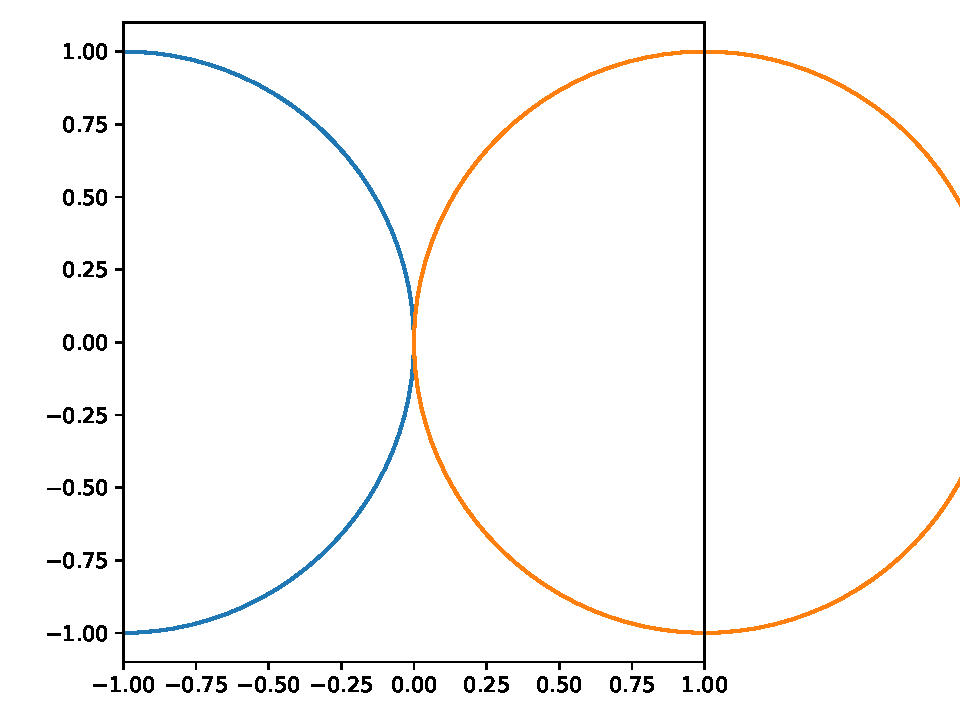
\includegraphics[width = .7\textwidth]{figures/proseplots/circle-clip.pdf}
\end{center}

\section{Axis Lines and Spines}\label{sec:axisSpines}

You might be used to plots that aren't surrounded by a box. Those enclosing lines, included by default, are called the \emph{spines}. The default might also be jarring if you're used to the typical $x$- and $y$-axis lines at $y=0$ and $x=0$, like in most math textbook plots. In this section we'll cover how to modify these. 

First, you might just eliminate everything with \code{ax.axis('off')}. We saw \code{plt.axis('off)} used similarly in Chapter \ref{chapter:oop} with a program that alternated between pyplot functions and the object-oriented approach. Below is a simple plot, empty but for a title, that becomes even emptier by eliminating the axis lines and labels. For reference, on the right is the same plot if \code{ax.axis('off')} were excluded from the program. 


\pyfile{no-axis.py}

\begin{center}
    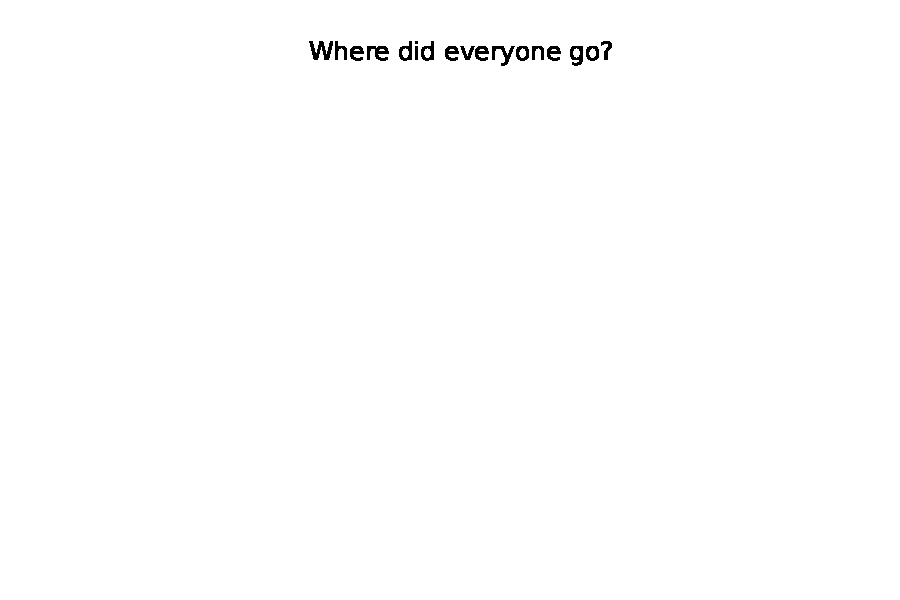
\includegraphics[width = .45\textwidth]{figures/proseplots/no-axis.pdf}   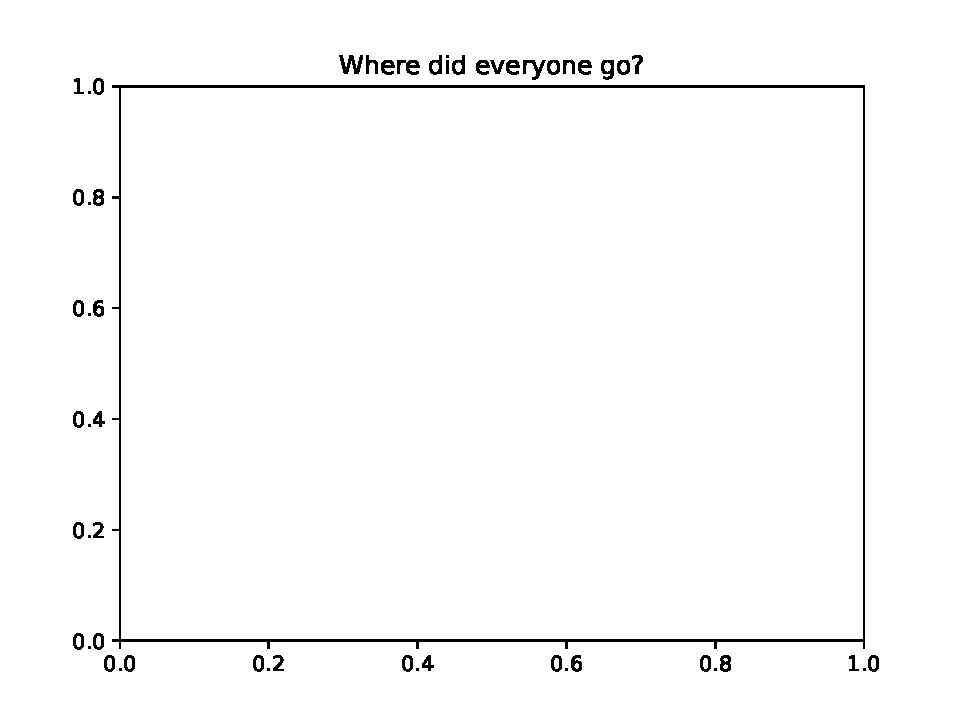
\includegraphics[width = .45\textwidth]{figures/proseplots/yes-axis.pdf}  %\caption{Caption}
\end{center}


Next, we can access and modify specific spines through \code{ax.spines}, which returns an \code{OrderedDict}. Access a specific spine using the appropriate key: \code{"left"}, \code{"right"}, \code{"top"}, or \code{"bottom"}.
A spine can be toggled on or off by passing the appropriate boolean value to \code{set_visible()}.

\pyfile{spine-vis.py}

\vspace{-0.2cm}
\begin{center}
    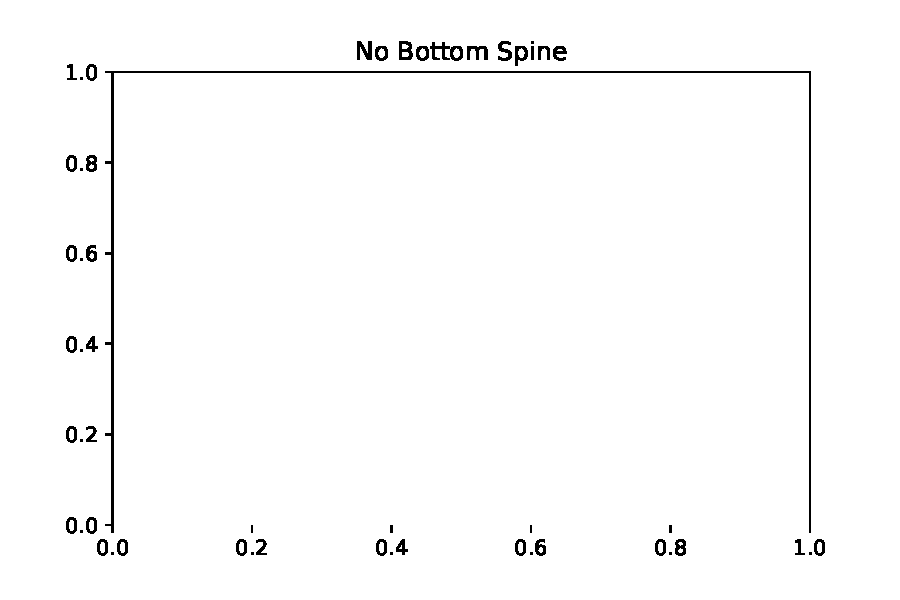
\includegraphics[width = 0.48\textwidth]{figures/proseplots/spine-vis-bottom.pdf} 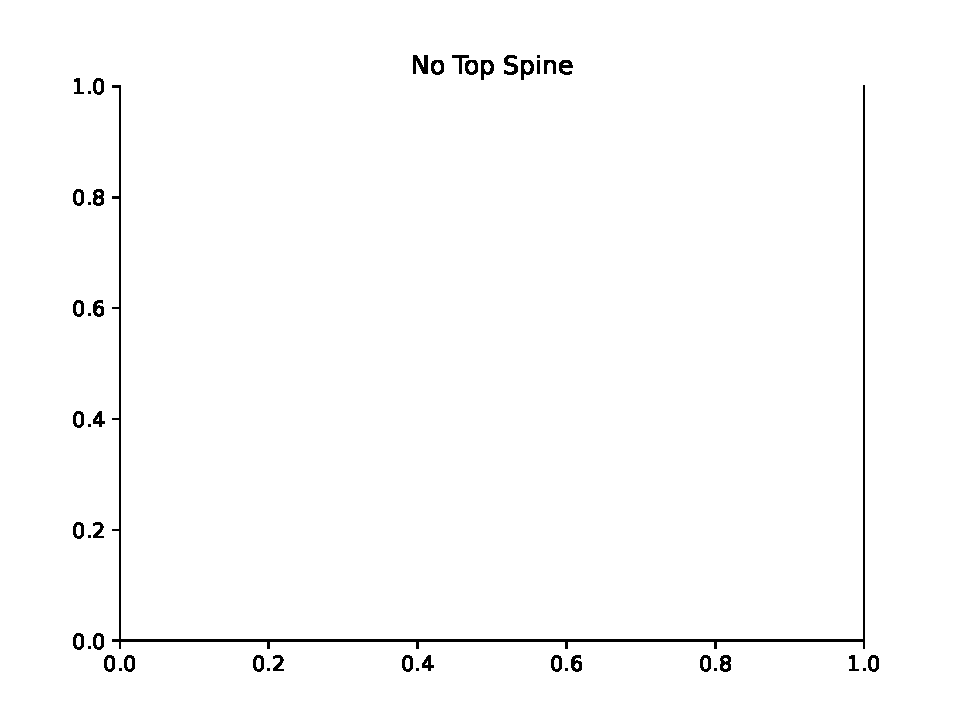
\includegraphics[width = 0.48\textwidth]{figures/proseplots/spine-vis-top.pdf}
    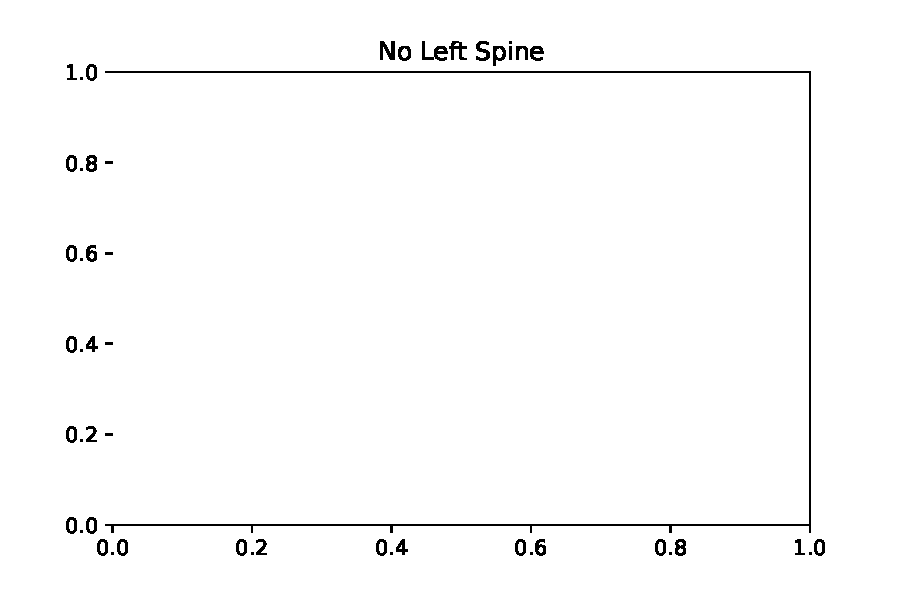
\includegraphics[width = 0.48\textwidth]{figures/proseplots/spine-vis-left} 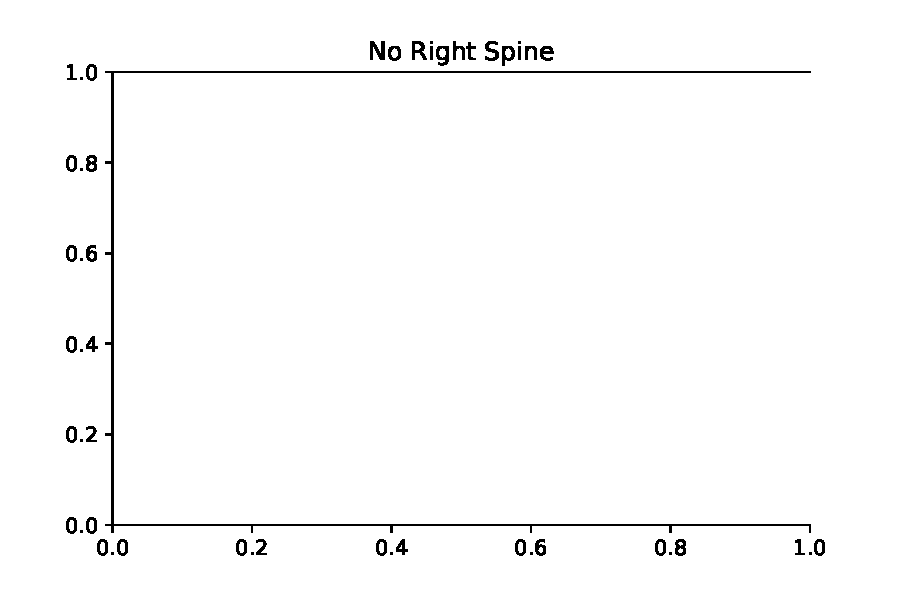
\includegraphics[width = 0.48\textwidth]{figures/proseplots/spine-vis-right.pdf}
\end{center}

Other spine modifications might be their width and color. Again, we access a particular spine and then make use of setter methods, \code{set_color} and \code{set_linewidth} in particular. 

\pyfile{thick-spines.py}
\begin{center}
    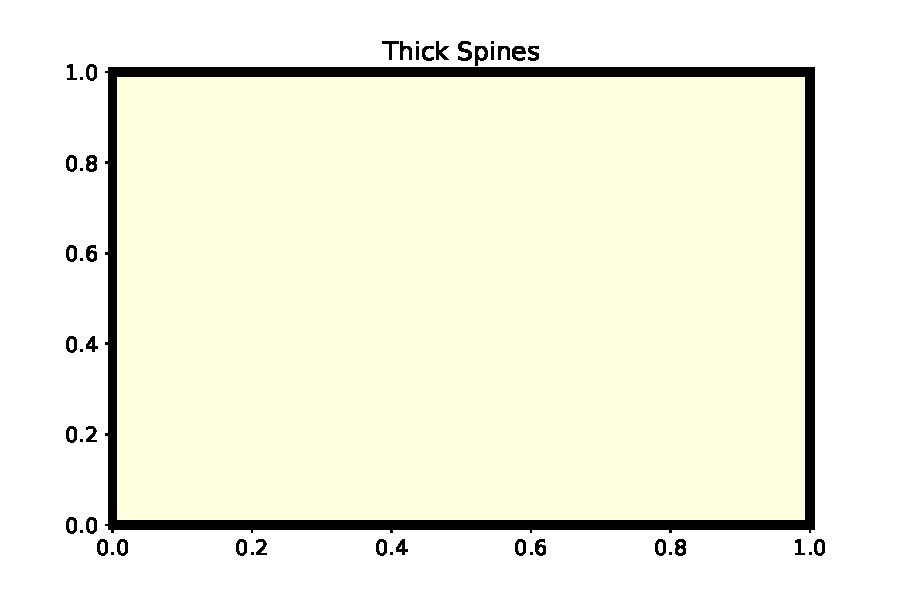
\includegraphics[width = .7\textwidth]{figures/proseplots/thick-spines.pdf}
\end{center}

It's easy to get this far imagining that spines are simply the pieces of the box enclosing your plot. But they don't have to enclose the plot if we alter them with the \code{set_position} method. Below, we set the bottom spine to be along the usual $x$-axis and the left spine to be along the usual $y$-axis by passing \code{'zero'} to \code{set_position}. The right and top spines are removed. 

\pyfile{zero-spines.py}

\begin{center}
    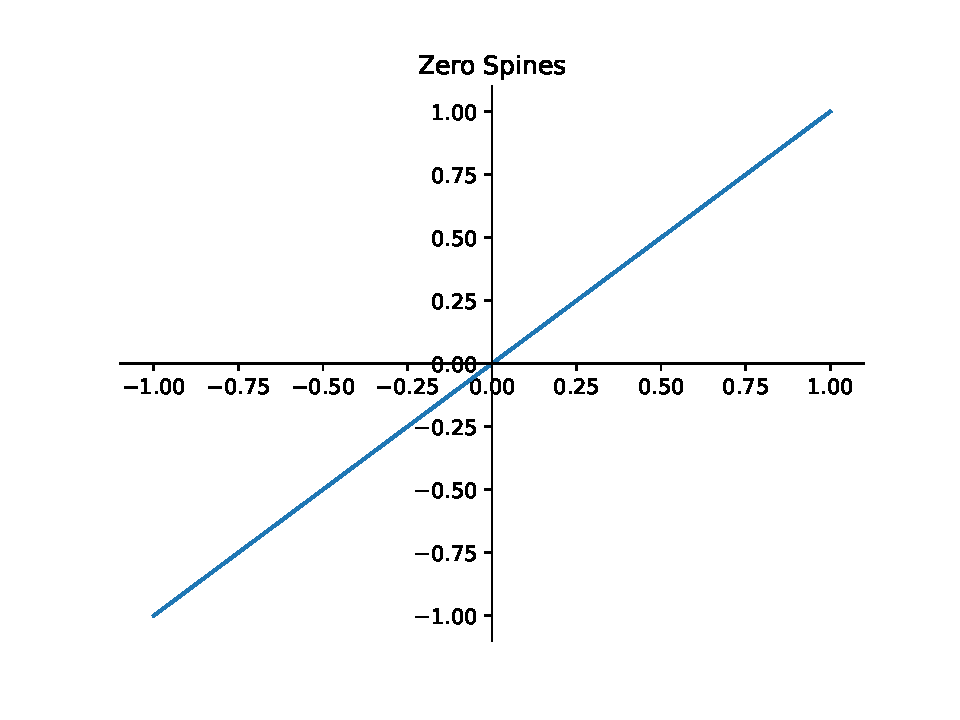
\includegraphics[width = .7\textwidth]{figures/proseplots/zero-spines.pdf}
\end{center}

We can go a step further and add arrows at the ends of our axis lines with some clever plotting. 
%https://matplotlib.org/stable/gallery/ticks_and_spines/centered_spines_with_arrows.html#sphx-glr-gallery-ticks-and-spines-centered-spines-with-arrows-py

\pyfile{arrow-axes.py}

\begin{center}
    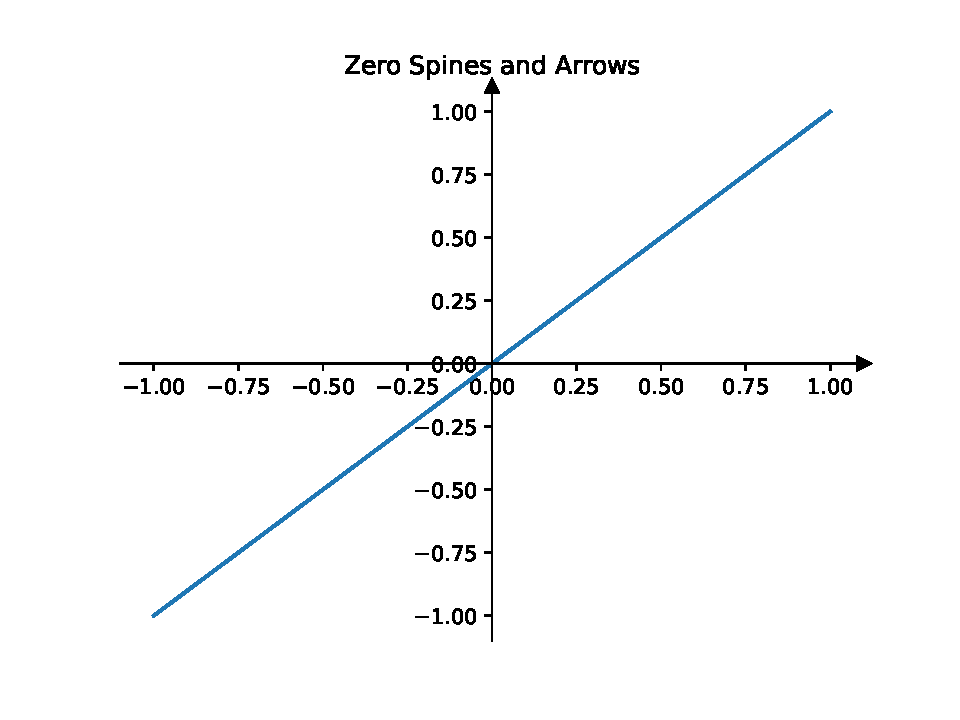
\includegraphics[width = .7\textwidth]{figures/proseplots/arrow-axes.pdf}
\end{center}

The tick labels do clutter the graph above. This can be solved after we cover Section \ref{sec:ticks}. \cite{knaflic2015storytelling} recommends removing the top and right spines as part of the imperative to declutter and remove unnecessary chart border. I think it is arguable. I'm used to default spines enclosing the data. Removing them can seem untidy, like the plot guts might spill out onto the page, or as if the plot is now vulnerable to intruders without any fencing. Arrows on axis lines subtly prod the reader to imagine what happens outside of the plotted region. I don't like that if, for example, I don't want to create the impression that a linear trend in a time series graph will continue into the future. 
% I also like that borders might subtly lessen your tendency to imagine the trend continuing beyond the axis limits. 
% see George Cumberland and William blake thoughts on outline
% page 33 from Blake biog Eternity's Sunrise


\section{Ticks}\label{sec:ticks}
%% Add something about ticks on the right for time series??

The important axes methods for ticks are \code{set_xticks}, \code{set_xticklabels}, and the natural $y$-axis counterparts. One may also use the general \code{set_ticks} and \code{set_ticklabels} with \code{ax.xaxis} or \code{ax.yaxis}---as axis (not axes) methods. These are demonstrated below, taking an array of tick locations and then the corresponding labels. I use \LaTeX strings to label the ticks. Here, that allows for a prettier $y$-axis, using fractions instead of decimals for tick labels. And on the $x$-axis, we can give a proper label of $\pi$ at $x = \pi$.

\pyfile{ticks1.py}

\begin{center}
    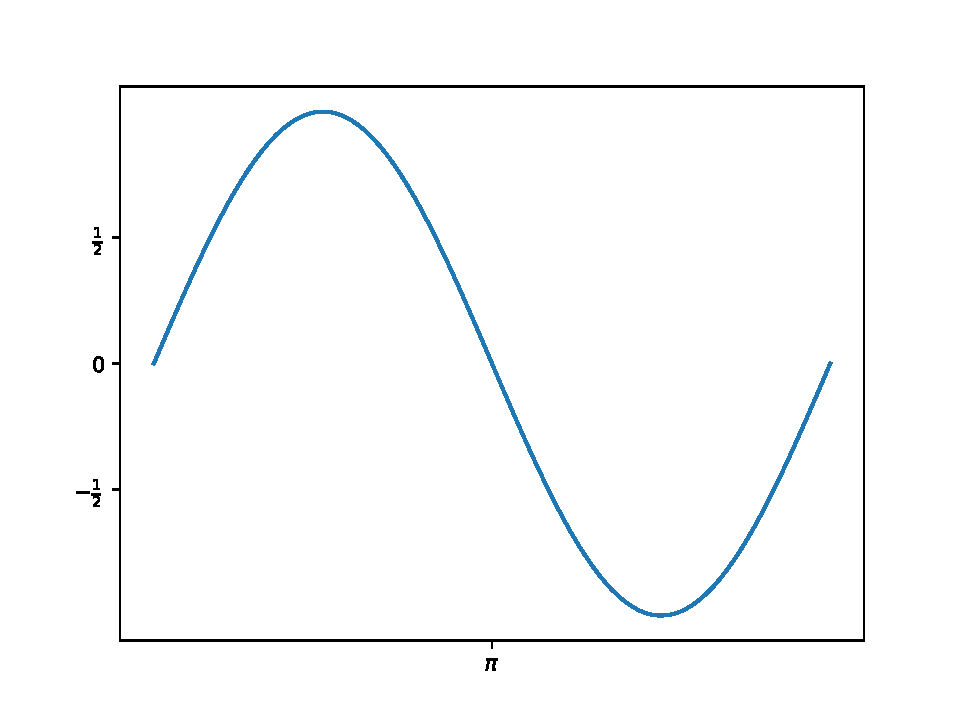
\includegraphics[width = .75\textwidth]{figures/proseplots/ticks1.pdf}
\end{center}

To remove the ticks entirely, simply pass an empty array to \code{set_ticks()}. To customize the appearance of your axis ticks and the labels, use the \code{set_tick_params} axis method. Parameters include \code{direction}, \code{width}, \code{length}, \code{color}, \code{pad}, \code{rotation}, \code{labelsize}, \code{labelcolor}

Imagine a measuring ruler, with ticks for every inch and smaller ticks at smaller intervals. So far our ticks have lacked that level of depth, but in fact we can work with two tick levels in matplotlib, major and minor ticks. Minor ticks are not shown by default. 

To start exploring these further customizations, you'll need to import additional formatters and or locators. For the below, you must import \code{MultipleLocator}, running \code{from matplotlib.ticker import MultipleLocator}.

\pyfile{tall-ballers.py}

\begin{center}
    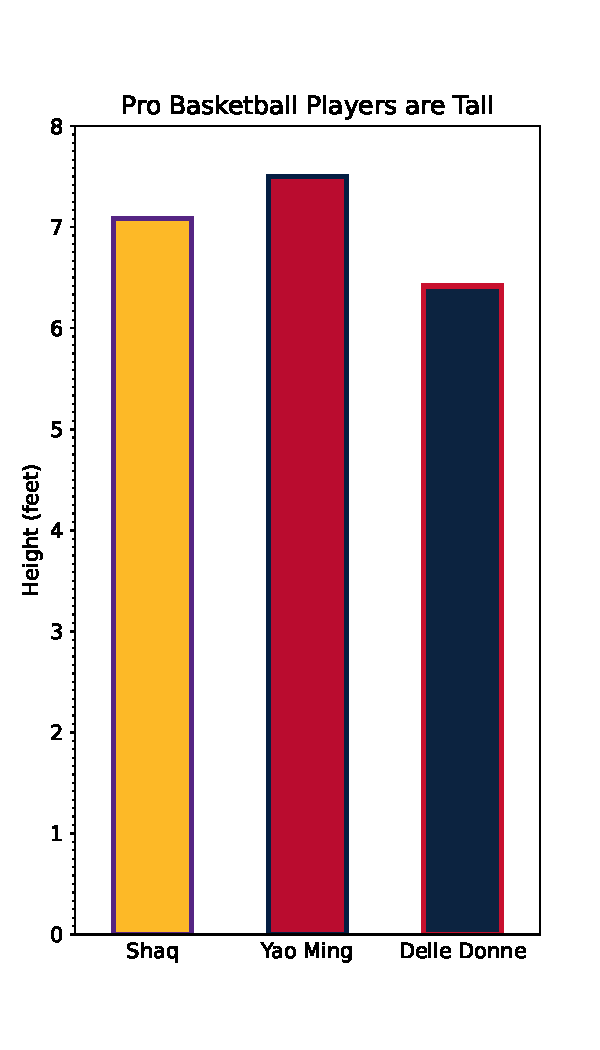
\includegraphics[width = .6\textwidth]{figures/proseplots/tall-ballers.pdf}
\end{center}

Major ticks can easily be set with \code{set_ticks} and its variants. Still, \code{MultipleLocator} and other locators are useful for setting major ticks without fooling with the details of the axes limits. 

With a function like $\sin x$, ticks might most naturally be placed at multiples of $\pi$. This can be accomplished by the below.

\pyfile{mult-locator.py}
\begin{center}
    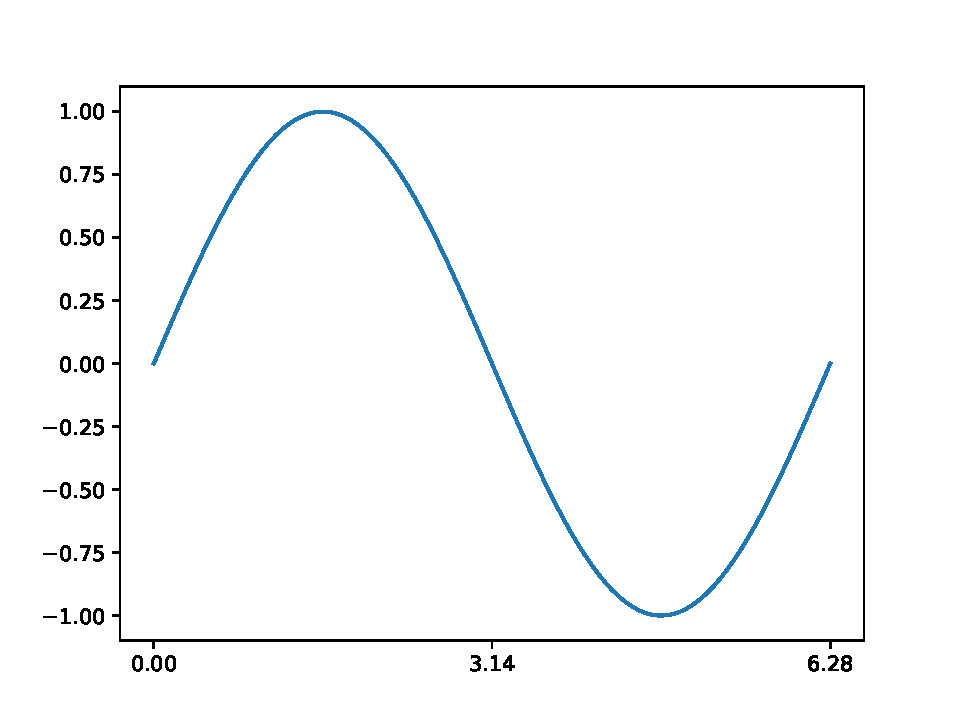
\includegraphics[width = .6\textwidth]{figures/proseplots/mult-locator.pdf}
\end{center}


It's true you could avoid the complication of locator classes by just using \code{ax.set_xticks([0, np.pi, 2*np.pi])}. For a plot this simple, do that. Suppose, you put ticks up to $3\pi$ though. Then you've extended the $x$-axis limit of the plot past your data. So you need to know your data to make the right tick adjustments by hand. If you'll be using the same code with different datasets, it'll be easier to use the details-free \code{MultipleLocator} and you can still rely on limit defaults or adjust them independently. 

Next, you might want to change the positioning of the ticks. By default $x$-axis ticks are on the bottom and $y$-axis ticks are on the left. You can modify these positions with axis methods. In time series data, for example, you might prefer to have the $y$-axis ticks on the right. Time marches on to the right and placing your ticks on the right can help emphasize that movement. This can be done with \code{set_ticks_position('right')} or the more concise \code{tick_right()}. The latter also accepts arguments of \code{'left'}, \code{'bottom'}, and \code{'top'}. Each has an abbreviated method like \code{tick_left()}. 

\pyfile{tick-right.py}

\begin{center}
    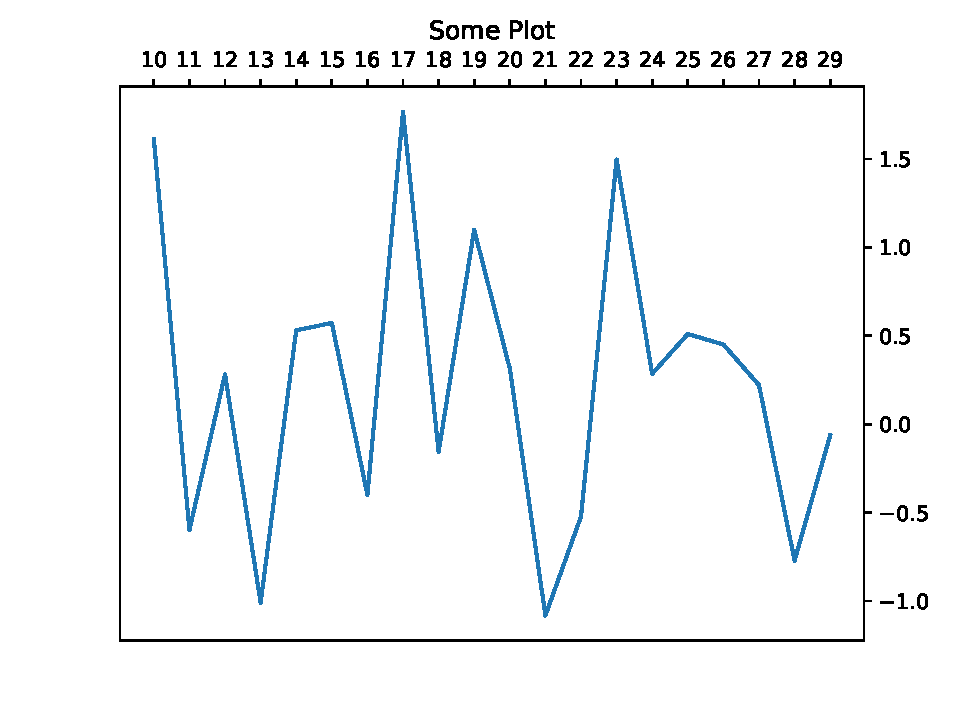
\includegraphics[width = .7\textwidth]{figures/proseplots/tick-right.pdf}
\end{center}

\section{Grids}

Including gridlines in a plot is generally discouraged (\cite{knaflic2015storytelling}, \cite{schwabish2021better}). It's clutter that won't spark joy. Perhaps we could stop here, with the instruction to run \code{ax.grid(False)} as in the code below (or rely on a style, like the default, that does this automatically).

\pyfile{grid-false.py}

\begin{center}
    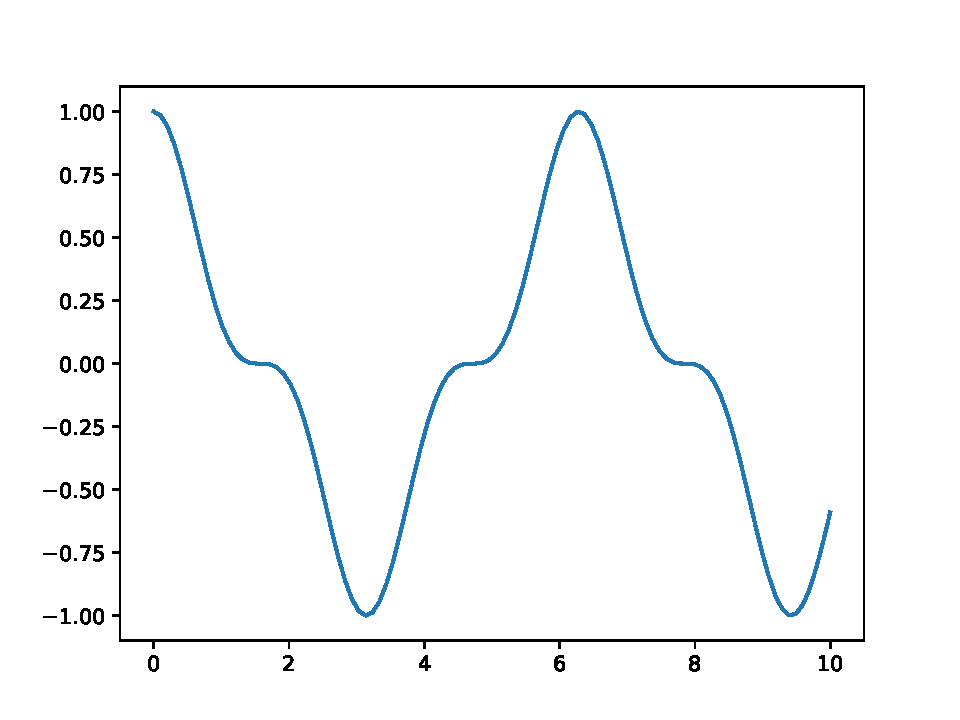
\includegraphics[width = .8\textwidth]{figures/proseplots/grid-false.pdf}
\end{center}

\noindent This does seem preferable to the following, but it's hardly an abomination. 

\pyfile{grid-true.py}

\begin{center}
    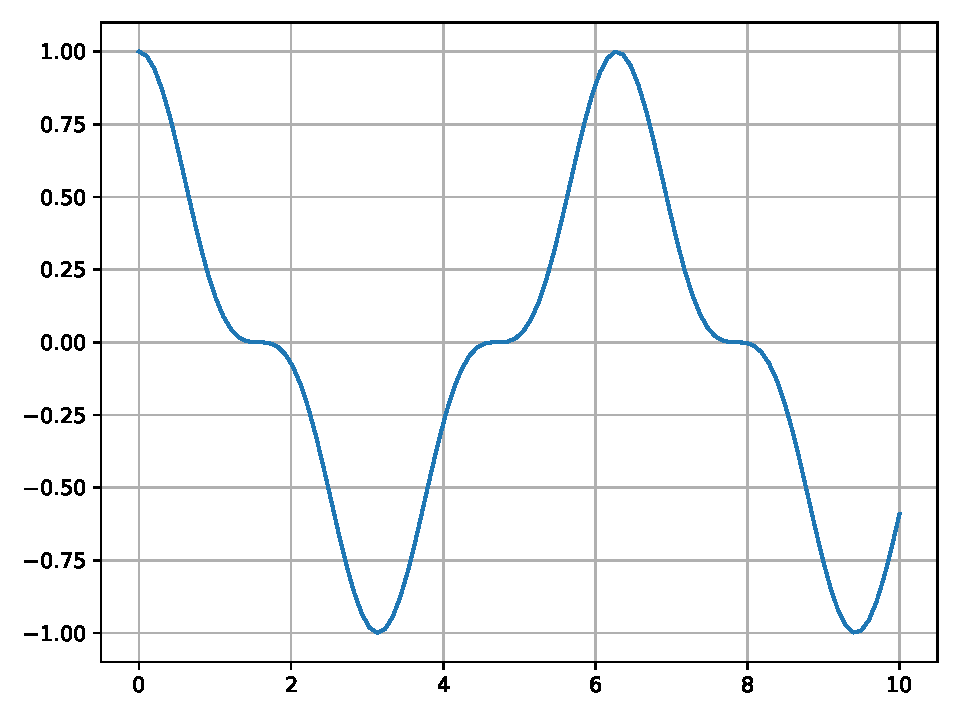
\includegraphics[width = .8\textwidth]{figures/proseplots/grid-true.pdf}
\end{center}

As a compromise, you might include gridlines for a single axis. If you want to emphasize that there is a slight trend in the data, then $y$-axis gridlines can help bring that pattern to the eye. Below we plot plots with and without a line of best fit and gridlines. Axis gridlines can be toggled independently by using \code{ax.xaxis.grid()} and \code{ax.yaxis.grid()}. 

\pyfile{y-grid-false.py}

\pyfile{y-grid-true.py}

\begin{center}
    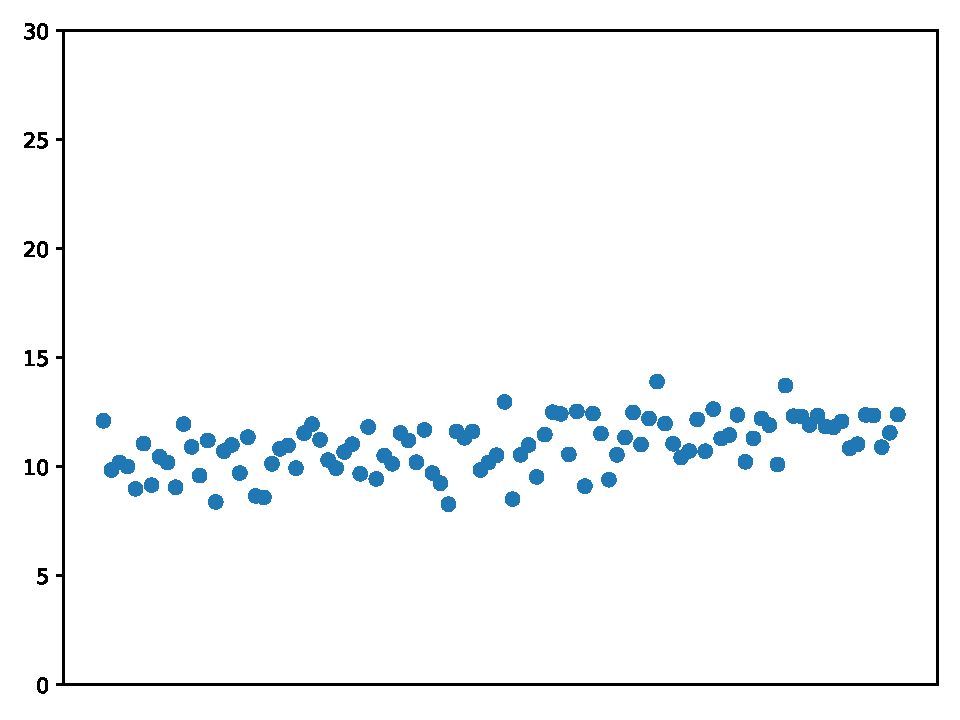
\includegraphics[width = .48\textwidth]{figures/proseplots/y-grid-false.pdf}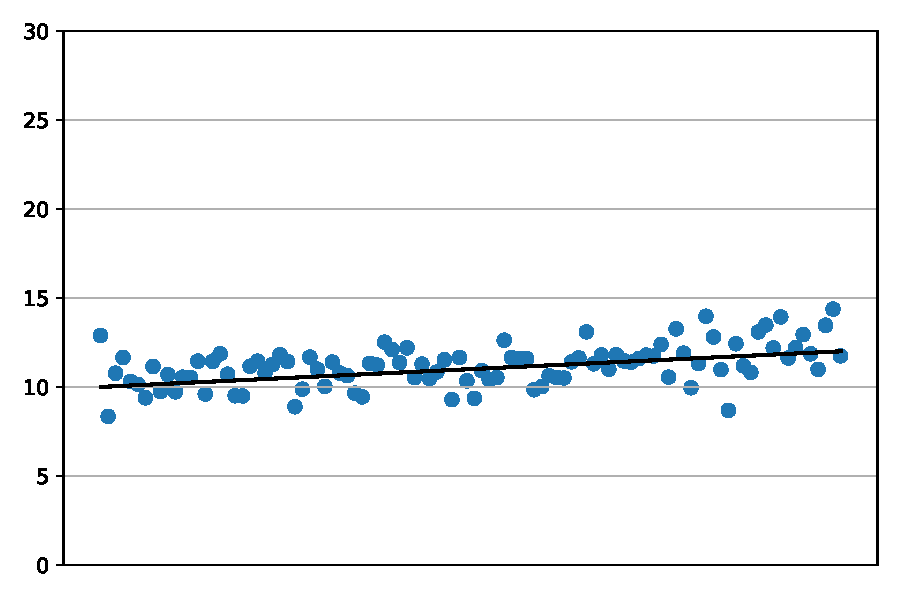
\includegraphics[width = .48\textwidth]{figures/proseplots/y-grid-true.pdf}
\end{center}



What we learned previously about locating ticks in Section \ref{sec:ticks} can be reapplied here, as seen in the examples further below. The location of gridlines and ticks can be set by the \code{set_major_locator()} and \code{set_minor_locator()} methods. \code{ax.grid()} is used to display the gridlines, but note it features a parameter \code{which}. The default value of \code{which} is \code{'major'}. To include minor gridlines, those minor ticks must be explicitly created (at least in the default style) and then the gridlines must be toggled on with \code{ax.grid(True, which = 'minor')} or for a single axis with \code{ax.xaxis.grid(True, which = 'minor')} for example. 


\pyfile{grids-auto.py}

\begin{center}
    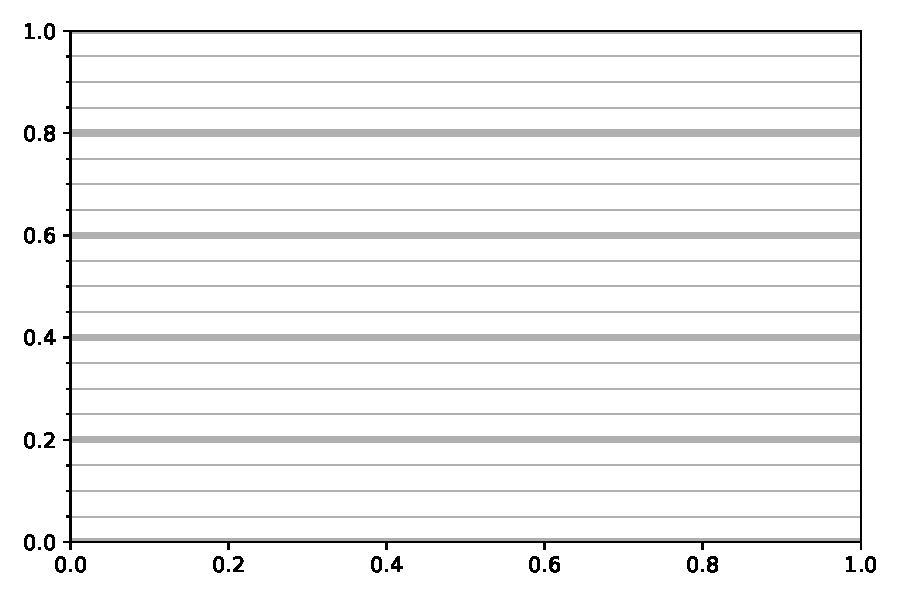
\includegraphics[width = .8\textwidth]{figures/proseplots/grids-auto.pdf}
\end{center}

\pyfile{grids-multi.py}

\begin{center}
    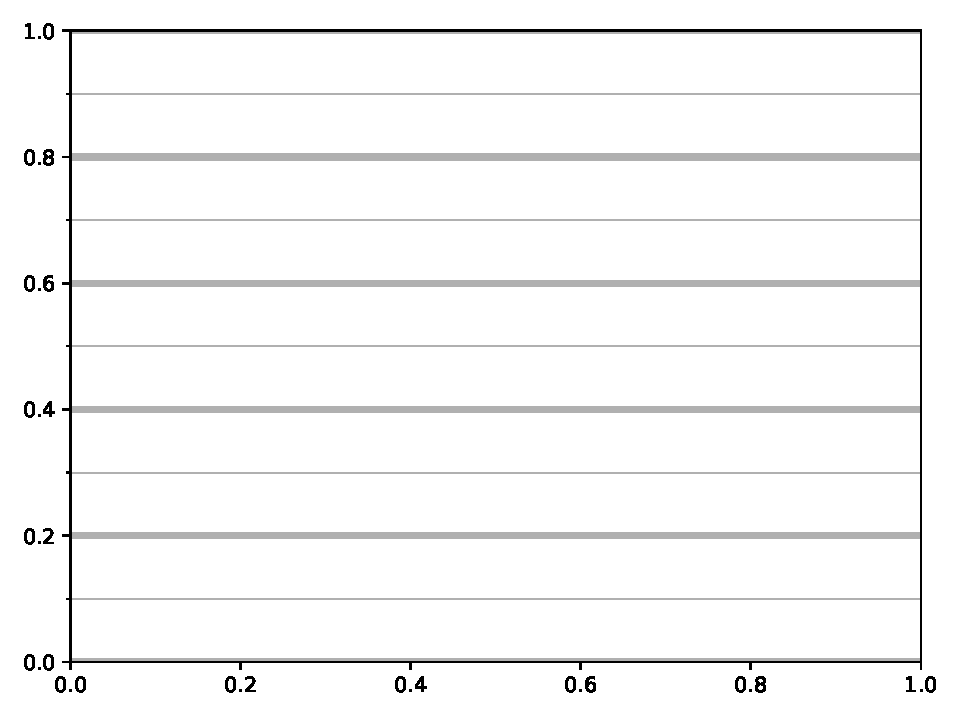
\includegraphics[width = .8\textwidth]{figures/proseplots/grids-multi.pdf}
\end{center}



%\section{Coordinates}